\documentclass[12pt,a4paper]{report}

\usepackage[utf8]{inputenc} % pentru suport diacritice
\usepackage[english]{babel} % setări pentru limba engleza 
\renewcommand\familydefault{\sfdefault} % sans serif

\usepackage[margin=2.54cm]{geometry}	% dimensiuni pagină și margini
\usepackage{graphicx} % support the \includegraphics command and options

% formatting sections and subsections
\usepackage{textcase}
\usepackage{hyphenat}
\usepackage[titletoc, title]{appendix}
\usepackage{titlesec}
\titleformat{\chapter}{\large\bfseries\MakeUppercase}{\thechapter}{2ex}{}[\vspace*{-1.5cm}]
\titleformat*{\section}{\large\bfseries}
\titleformat*{\subsection}{\large\bfseries}
\titleformat*{\subsubsection}{\large\bfseries}

\usepackage{chngcntr}
\counterwithout{figure}{chapter} % no chapter number in figure labels
\counterwithout{table}{chapter} % no chapter number in table labels
\counterwithout{equation}{chapter} % no chapter number in equation labels

\usepackage{booktabs} % for much better looking tables
\usepackage{url} % Useful for inserting web links nicely
\usepackage[bookmarks,
			unicode,
			hidelinks,
			colorlinks = true,
			anchorcolor = blue,
			linkcolor = black,
			urlcolor = blue]{hyperref}

\usepackage{array} % for better arrays (eg matrices) in maths
\usepackage{paralist} % very flexible & customisable lists (eg. enumerate/itemize, etc.)
\usepackage{verbatim} % adds environment for commenting out blocks of text & for better verbatim
\usepackage{subfig} % make it possible to include more than one captioned figure/table in a single float
\usepackage{enumitem}
\setlist{noitemsep}

%%% HEADERS & FOOTERS
\usepackage{fancyhdr}
\pagestyle{empty}
\renewcommand{\headrulewidth}{0pt}
\renewcommand{\footrulewidth}{0pt}
\lhead{}\chead{}\rhead{}
\lfoot{}\cfoot{\thepage}\rfoot{}



\newcommand{\HeaderLineSpace}{-0.25cm}
\newcommand{\UniTextRO}{UNIVERSITATEA POLITEHNICA DIN BUCUREȘTI \\[\HeaderLineSpace] 
FACULTATEA DE AUTOMATICĂ ȘI CALCULATOARE \\[\HeaderLineSpace]
DEPARTAMENTUL DE CALCULATOARE\\}
\newcommand{\DiplomaRO}{PROIECT DE DIPLOMĂ}
\newcommand{\AdvisorRO}{Coordonator științific:}
\newcommand{\BucRO}{BUCUREȘTI}

\newcommand{\UniTextEN}{UNIVERSITY POLITEHNICA OF BUCHAREST \\[\HeaderLineSpace]
FACULTY OF AUTOMATIC CONTROL AND COMPUTERS \\[\HeaderLineSpace]
COMPUTER SCIENCE AND ENGINEERING DEPARTMENT\\}
\newcommand{\DiplomaEN}{DIPLOMA PROJECT}
\newcommand{\AdvisorEN}{Thesis advisor:}
\newcommand{\BucEN}{BUCHAREST}

\newcommand{\frontPage}[6]{
\begin{titlepage}
\begin{center}
{\Large #1}  % header (university, faculty, department)
\vspace{50pt}
\begin{tabular}{p{6cm}p{4cm}}

\includegraphics[scale=0.8]{pics/upb-logo.jpg} &
	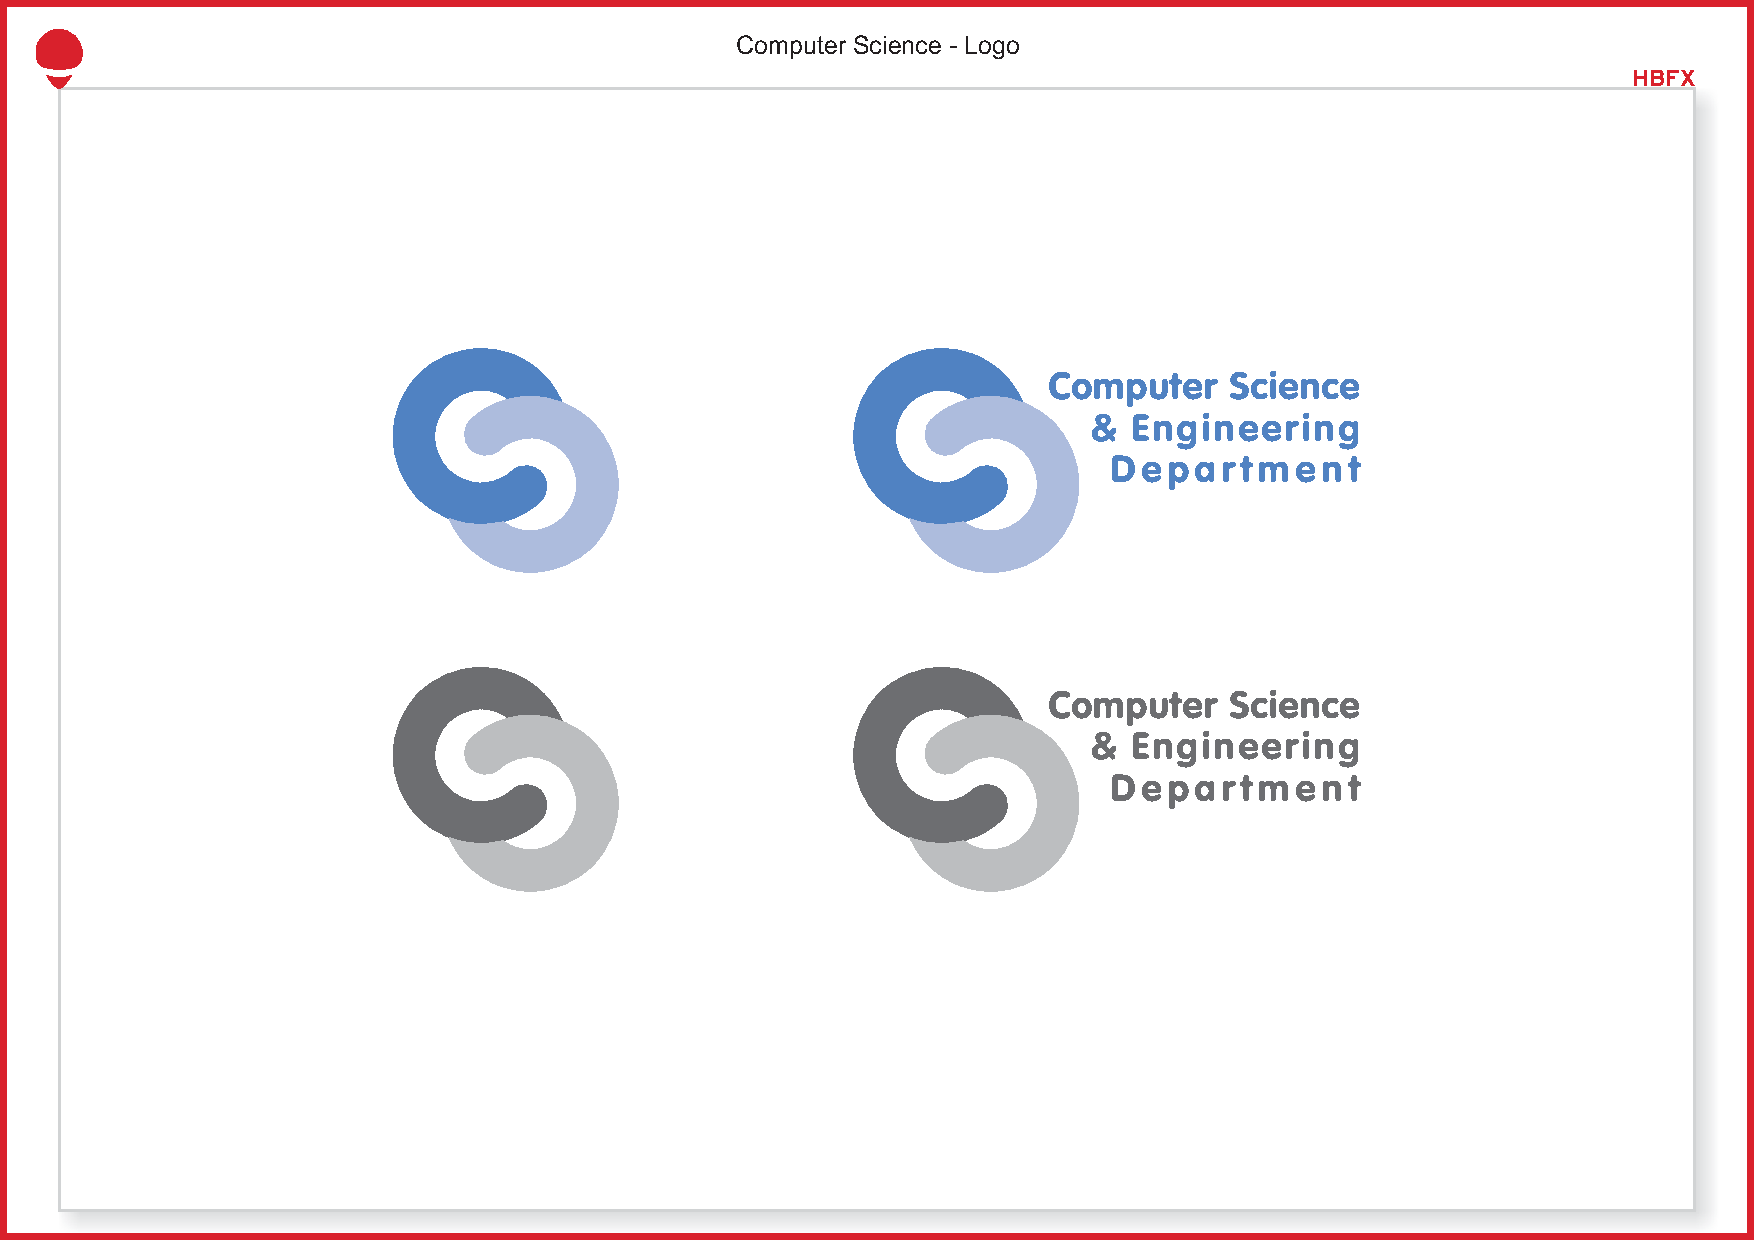
\includegraphics[scale=0.5,trim={14cm 11cm 2cm 5cm},clip=true]{pics/cs-logo.pdf}
\end{tabular}

\vspace{105pt}
{\Huge #2}\\                           % diploma project text
\vspace{40pt}
{\Large #3}\\ \vspace{0pt}  % project title
{\Large #4}\\                          % project subtitle
\vspace{40pt}
{\LARGE \Name}\\                   % student name
\end{center}
\vspace{60pt}
\begin{tabular*}{\textwidth}{@{\extracolsep{\fill}}p{6cm}r}
&{\large\textbf{#5}}\vspace{10pt}\\      % scientific advisor
&{\large \Advisor}                                    % advisor name
\end{tabular*}
\vspace{20pt}
\begin{center}
{\large\textbf{#6}}\\                                % bucharest
\vspace{0pt}
{\normalsize \Year}
\end{center}
\end{titlepage}
}

\newcommand{\frontPageRO}{\frontPage{\UniTextRO}{\DiplomaRO}{\ProjectTitleRO}{\ProjectSubtitleRO}{\AdvisorRO}{\BucRO}}
\newcommand{\frontPageEN}{\frontPage{\UniTextEN}{\DiplomaEN}{\ProjectTitleEN}{\ProjectSubtitleEN}{\AdvisorEN}{\BucEN}}

\linespread{1.15}
\setlength\parindent{0pt}
\setlength\parskip{.28cm}

%% Abstract macro
\newcommand{\AbstractPage}{
\begin{titlepage}
\textbf{\large SINOPSIS}\par
\AbstractRO\par\vfill
\textbf{\large ABSTRACT}\par
\AbstractEN \vfill
\end{titlepage}
}

%% Thank you macro
\newcommand{\ThanksPage}{
\begin{titlepage}
{\noindent \large\textbf{MULȚUMIRI}}\\
\Thanks
\end{titlepage}
}



%%%%%%%%%%%%%%%%%%%%%%%%%%%%%%%%%%%%%%%%%%%%%%%%%%   
%%
%%          End of template definitions
%%   
%%%%%%%%%%%%%%%%%%%%%%%%%%%%%%%%%%%%%%%%%%%%%%%%%%


%%% Puteți elimina aceste linii din lucrare, servesc numai pentru template.
\newcommand{\worktype}[1]{[\textit{#1}] }
\newcommand{\dezvoltare}{\worktype{Dezvoltare de produs}}
\newcommand{\cercetare}{\worktype{Cercetare}}
\newcommand{\ambele}{\worktype{Ambele}}
\newcommand{\website}{\href{https://acadnet.dev}{AcadNet.dev}}
%%%


%%
%%   Campurile de mai jos trebuie modificate de autor. Modificati doar continutul, nu si numele fiecarei definitii
%%
\newcommand{\ProjectTitleRO}{AcadNet.dev}
\newcommand{\ProjectSubtitleRO}{Platformă online pentru rezolvarea problemelor de informatică}
\newcommand{\ProjectTitleEN}{AcadNet.dev}
\newcommand{\ProjectSubtitleEN}{Online platform for solving computer science problems}
\newcommand{\Name}{Dimitrie David}
\newcommand{\Advisor}{Prof. Dr. Ing. Răzvan Victor Rughiniș }
\newcommand{\Year}{2023}

% Setări document
\title{Proiect de diplomă}
\author{\Name}
\date{\Year}

%%
%%   Campurile aferente rezumatului
%%
\newcommand{\AbstractRO}{Această lucrare prezintă \website, o platformă online pentru rezolvarea de probleme de informatică. Platforma oferă un mediu de lucru complet, care permite utilizatorilor să creeze probleme, să le rezolve și să le evalueze automat. Platforma oferă și un mediu de lucru online, care permite utilizatorilor să rezolve problemele direct în browser, fără a fi nevoie să instaleze un mediu de dezvoltare local.}

\newcommand{\AbstractEN}{This paper presents \website, an online platform for solving computer science problems. The platform provides a complete working environment, which allows users to create problems, solve them and automatically evaluate them. The platform also provides an online working environment, which allows users to solve problems directly in the browser, without the need to install a local development environment.}

%%
%%   Campurile aferente paginii de multumiri
%%
\newcommand{\Thanks}{(opțional) Aici puteți introduce o secțiunea specială de mulțumiri / acknowledgments. }

\begin{document}

\frontPageRO
\frontPageEN

\begingroup
\linespread{1}
\tableofcontents
\endgroup

\AbstractPage

% poate fi comentata sau stearsa
\ThanksPage


% Textul licentei incepe de aici 


% INRODUCTION
\chapter{Introduction}\pagestyle{fancy}
\section{Background and motivation}

\section{Problem statement}

\section{Objectives}

\section{Proposed solution and achieved results}



% PROPOSED SOLUTION
\chapter{System design and architecture}
\section{User journey}

\section{Architecture overview}

\section{System components and interactions}

\section{Database design}



% IMPLEMENTATION DETAILS
\chapter{Implementation details}
\section{Web application}

\section{SQL database}

\section{File storage}

\section{Checker}

\section{VSCode workspaces}



% FEATURES AND FUNCTIONALITIES
\chapter{Features and functionalities}
\section{User authentication}

\section{Problem creation}

\section{Problem browsing}

\section{Problem solving}

\section{Submission evaluation}

\section{Online workspaces}



% DEPLOYMENT AND MAINTENANCE
\chapter{Deployment and maintenance}
\section{Infrastructure}

\section{Continuous integration}

\section{Continuous deployment}

\section{Monitoring}



% TESTING AND VALIDATION
\chapter{Testing and validation}
\section{Evaluation criteria}

\section{Performance}

\section{Security}

\section{User feedback}



% CONCLUSIONS AND FUTURE WORK
\chapter{Conclusions and future work}
\section{Conclusions}

\section{Future enhancements}

\section{Lessons learned}



% BIBLIOGRAPHY
\chapter*{Bibliography}\addcontentsline{toc}{chapter}{Bibliography}  
% * <marios.choudary@gmail.com> 2018-02-28T12:07:48.730Z:
% 
% > BIBLIOGRAFIE
% Am adaugat un paragraf cu cateva detalii despre folosirea citarilor bibliografice in Latex, despre folosirea lui "\cite" si despre posibilitatea folosirii bibliografiei si direct in fisierul Latex.
% 
% ^.

\begin{itemize}
	\item 	NU utilizați referințe la Wikipedia sau alte surse fără autor asumat.
	\item 	Pentru referințe la articole relevante accesibile în web (descrise prin URL) se va nota la bibliografie și data accesării.
	\item 	Mai multe detalii despre citarea referințelor din internet se pot regăsi la:
	\begin{itemize}
		\item	\url{http://www.writinghelp-central.com/apa-citation-internet.html}
		\item	\url{http://www.webliminal.com/search/search-web13.html}
	\end{itemize}
	\item 	Note de subsol se utilizează dacă referiți un link mai puțin semnificativ o singură dată; Dacă nota este citată de mai multe ori, atunci utilizați o referință bibliografică.
	\item 	Dacă o imagine este introdusă în text și nu este realizată de către autorul lucrării, trebuie citată sursa ei (ca notă de subsol sau referință - este de preferat utilizarea unei note de subsol).
	\item 	Referințele se pun direct legate de text (de exemplu ``KVM [1] uses'', ``as stated by Popescu and Ionescu [12]'', etc.). Nu este recomandat să folosiți formulări de tipul ``[1] uses'', ``as stated in [12]'', ``as described in [11]'' etc..
	\item 	Afirmațiile de forma ``are numerous'', ``have grown exponentially'', ``are among the most used'', ``are an important topic'' trebuie să fie acoperite cu citări, date concrete si analize comparative.
	\begin{itemize}
		\item	Mai ales în capitolele de introducere, ``state of the art'', ``related work'' sau ``background'' trebuie să vă argumentați afirmațiile prin citări. Fiți autocritici și gândiți-vă dacă afirmațiile au nevoie de citări, chiar și cele pe care le considerați evidente.
		\item	Cea mai mare parte dintre citări vor fi în capitolele de introducere ``state of the art'', ``related work'' sau ``background''.
	\end{itemize}
	\item 	Toate intrările bibliografice trebuie citate în text. Nu le adăugați pur și simplu la final.
	\item 	Nu copiați sau traduceți niciodată din surse de informație de orice tip (online, offline, cărți, etc.). Dacă totuși doriți să oferiți, prin excepție, un citat celebru - de maxim 1 frază- utilizați ghilimele și evident menționați sursa. .
	\item 	Dacă reformulați idei sau creați un paragraf rezumat al unor idei folosind cuvintele voastre, precizați cu citare (referință bibliografică) sau cu notă de subsol sursa sau sursele de unde ați preluat ideile.
\end{itemize}

Trebuie respectat un singur standard de trimiteri bibliografice (citare), dintre următoarele alternative:
\begin{itemize}
	\item APA (\url{http://pitt.libguides.com/c.php?g=12108\&p=64730})
	\item IEEE (\url{https://ieee-dataport.org/sites/default/files/analysis/27/IEEE\%20Citation\%20Guidelines.pdf}) 
	\item Harvard (\url{https://libweb.anglia.ac.uk/referencing/harvard.htm})
	\item Cu numerotarea referințelor în ordine alfabetică sau în ordinea apariției în text (de exemplu, stilul cu numere folosit de unele publicații ACM - \url{https://www.acm.org/publications/authors/reference-formatting}) 
\end{itemize}

În Latex este foarte ușor să folosiți referințe într-un mod corect și unitar, fie prin adăugarea unei secțiuni
\verb!\begin{thebibliography}!
(vezi la sfârșitul acestei secțiuni), fie printr-un fișier separat de tip bib, folosind comanda
\verb!\bibliography{}!,
așa cum procedăm mai jos prin folosirea fișierului ``bibliography.bib''. În orice caz, în Latex va trebui să folosiți comanda
\verb!\cite{}!
pentru a adăuga referințe, iar această comandă trebuie folosită direct în text, acolo unde vreți sa apară citația, ca în exemplele următoare:
\begin{itemize}
	\item Articol jurnal: ~\cite{article};
	\item Articol conferință:~\cite{proc};
	\item Carte: ~\cite{book};
	\item Weblink: ~\cite{silva};
\end{itemize}

\textbf{Important}: în această secțiune de obicei apar doar intrările bibliografice (adică doar listarea referințelor). Citarea lor prin comanda cite și explicații legate de ele trebuie facute în secțiunile anterioare. Citarea de mai sus a fost facută aici doar pentru exemplificare.

% Asa se specifica folosirea unui fisier cu referinte bibliografice:
\bibliographystyle{plain}
\bibliography{bibliography}

%% O alta varianta ar fi fost includerea de articole direct in acest fisier
%% in felul urmator:
%% \begin{thebibliography}{ABC}
%%
%% \bibitem{article}
%%  H. Baali, H. Djelouat, A. Amira and F. Bensaali,
%%  ``Empowering Technology Enabled Care Using IoT and Smart Devices:
%   A Review''. In: IEEE Sensors Journal, vol. 322 (10), pp. 891--921, 1905.
%%
%% (more \bibitem items here...)
%%
%% \end{thebibliography}

%% Daca vreti ca o sectiune sa inceapa pe o pagina noua, puteti forta acest lucru cu comanda "\newpage", ca mai jos:

%\newpage

\chapter*{Appendices}\addcontentsline{toc}{chapter}{Appendices}
\begin{appendices}

\chapter{Extrase de cod} % Introduce o nouă anexă
\ldots


\end{appendices}
\end{document}